\subsection{Functional requirement}
\begin{enumerate}
\item A client can register to the system by providing an e-mail, valid payment information and a photo of his driving license.
\begin{enumerate}
\item The system must be able to check the validity of the payment information.
\item The system must be able to check if the uploaded documents are in the accepted format.
\item The system must be able to communicate with the civil registry office and transport authority in order to obtain user profile information from ID number and license number. 
\item The system must allow the registration only if ID ,license and personal information are related to the same person.
\item The system must implement a retrieve password mechanism.
\item The system should not allow to complete the registration process to an already registered user.
\item The system should not allow different users to register with the same email.
\end{enumerate}

\item A client can log in into system.
\begin{enumerate}
\item The system should provide the log in function both in the app and the web application.
\item The system should allow to rent a car only after the log in.
\item The system must guarantee that none can access to a user profile without the right credentials.
\item The system must be able to check if the credentials inserted by the user are correct.
\item The system must deny the access to blocked users.
\end{enumerate}

\item Allows clients to obtain information about
the position of available cars(position and remaining charge), safe areas(boundaries) and charging stations (position and available plugs).
\begin{enumerate}
\item The system should acquire the GPS position of available cars.
\item The system must offer a view of a map in which are displayed the position the available cars and the charging stations and the boundaries of the safe areas.
\item The system should update in real time the information about the charging stations and available cars.
\item The system must detect the position of clients that have opened the application.
\end{enumerate}


\item Allows clients to reserve a car that fits most their needs.
\begin{enumerate}
\item  The system should not allow a client to reserve more than one car simultaneously.
\item The system must not show in on the map the car reserved. 
\item The system must delete automatically the reservation after 1 hour.
\item The system has to apply to the client a fee of 1 euro if the reservation lasts more than 1 hour.
\item The system has to permits to reserve only available cars that are shown in the map.
\item The system should provide to the client the possibility to cancel the reservation.
\item The system must set available a car when its reservation is canceled.
\item A user that cancel a reservation can't reserve the same car within 15 minutes from the cancellation.
\item The system must terminate the reservation when the client starts the rent.
\end{enumerate}


\item A client can start the rent opening a car that has reserved previously when he/she is in the near by.

\begin{enumerate}
\item The system should be able to know the user GPS position.
\item The system should permit a client to request the opening of a car if and only if there is an active reservation of that user for that car and the user GPS position is not farther than 15 meters from the car GPS position.
\item The system should make possible to start the engine if and only if the user have inserted the correct pin.
\item After the client authentication the system should provide a function to insert the destination and eventually select the saving mode option. 
\item The system must start the rent right after the car doors are unlocked.
\end{enumerate}

\item During the rent a client can display the amount of money charged.
\begin{enumerate}
\item The system must detect when the engine is on.
\item The system must count the passed minutes to calculate the current charge.
\item The system must refresh every minute the current cost of the rent.
\item The system must always show the current cost during the rent.
\item The system must stop charging when the user turn off the engine and selects the "end rent" option.
\item The system must detect the moment when the client finish the rent.
\end{enumerate}

\item Guarantee as many available cars as possible encouraging clients to have a virtuous and eco-friendly behavior applying fees and discounts.
\begin{enumerate}
\item The system must apply  a discount of 10\% on the last ride if it detects that during the rent the user had at least other two passengers onto the car.
\item The system must apply a discount of 20 \% on the last ride if the client leaves the car with less than 50 \% of the battery empty.
\item The system must apply a discount of 30 \% on the last ride if the client plugs the car into the power grid of a charging station.
\item The system must charge 30 \% more on the last ride if the client leaves the car at more than 3 KM from the nearest charging station.
\item The system must charge 30 \% more on the last ride if the client leaves the car with a remaining charge of 20\% or less.
\end{enumerate}
	

\item Allows clients to end the rent and leave the car in any safe area.
\begin{enumerate}
\item The Display of the car system should provide a section that permits the user to end the rent.
\item The system should allow a client to end the rent if and only if the client clicks the "end rent" button and the car GPS position is inside a safe area.
\item After a minute from the end of the rent the system should lock the car doors.
\item After 5 minutes from the end of the rent the system will charge the rent cost, proportional to the duration of the ride and reduced by eventual discounts.
\item If the system tries to charge the user but the payment is unsuccessful the system blocks the log-in function of the user until the user doesn't absolve his debt. 
\end{enumerate}

\item Clients can report eventual damages made by users that have driven the car before.
\begin{enumerate}
\item The system must provide a section where the client can specify the entity of damage or the level of dirty.
\item The system must implement the possibility of communicate with an external operator system.
\item The system must allow the client to immediately finish the rent without apply any cost. 
\item The system should be able to find the last user that used a car.
\item The system must allow the client to not start the rent, without apply any penalties in case of damages.
\end{enumerate}

\item Clients can select a "saving money" option.
\begin{enumerate}
\item The system must provide the possibility to select the "saving option" during the rent.
\item When the saving money option is enabled the system must will information about the charging station, where to leave and plug the car, based on the destination selected, the availability of power plugs and the distribution of cars in the city.
\end{enumerate}
\end{enumerate}

\subsection{Non functional requirement}
Users can interact with our system through the mobile application, the website and the display located inside the car.

\subsubsection{View available car information in mobile application} This mockup shows how the information of an available car (charge level and distance from the client) can be displayed on the mobile app. The logged client has the possibility to reserve the car by tapping on the "Reserve" button.
\begin{figure}[h]
\centering
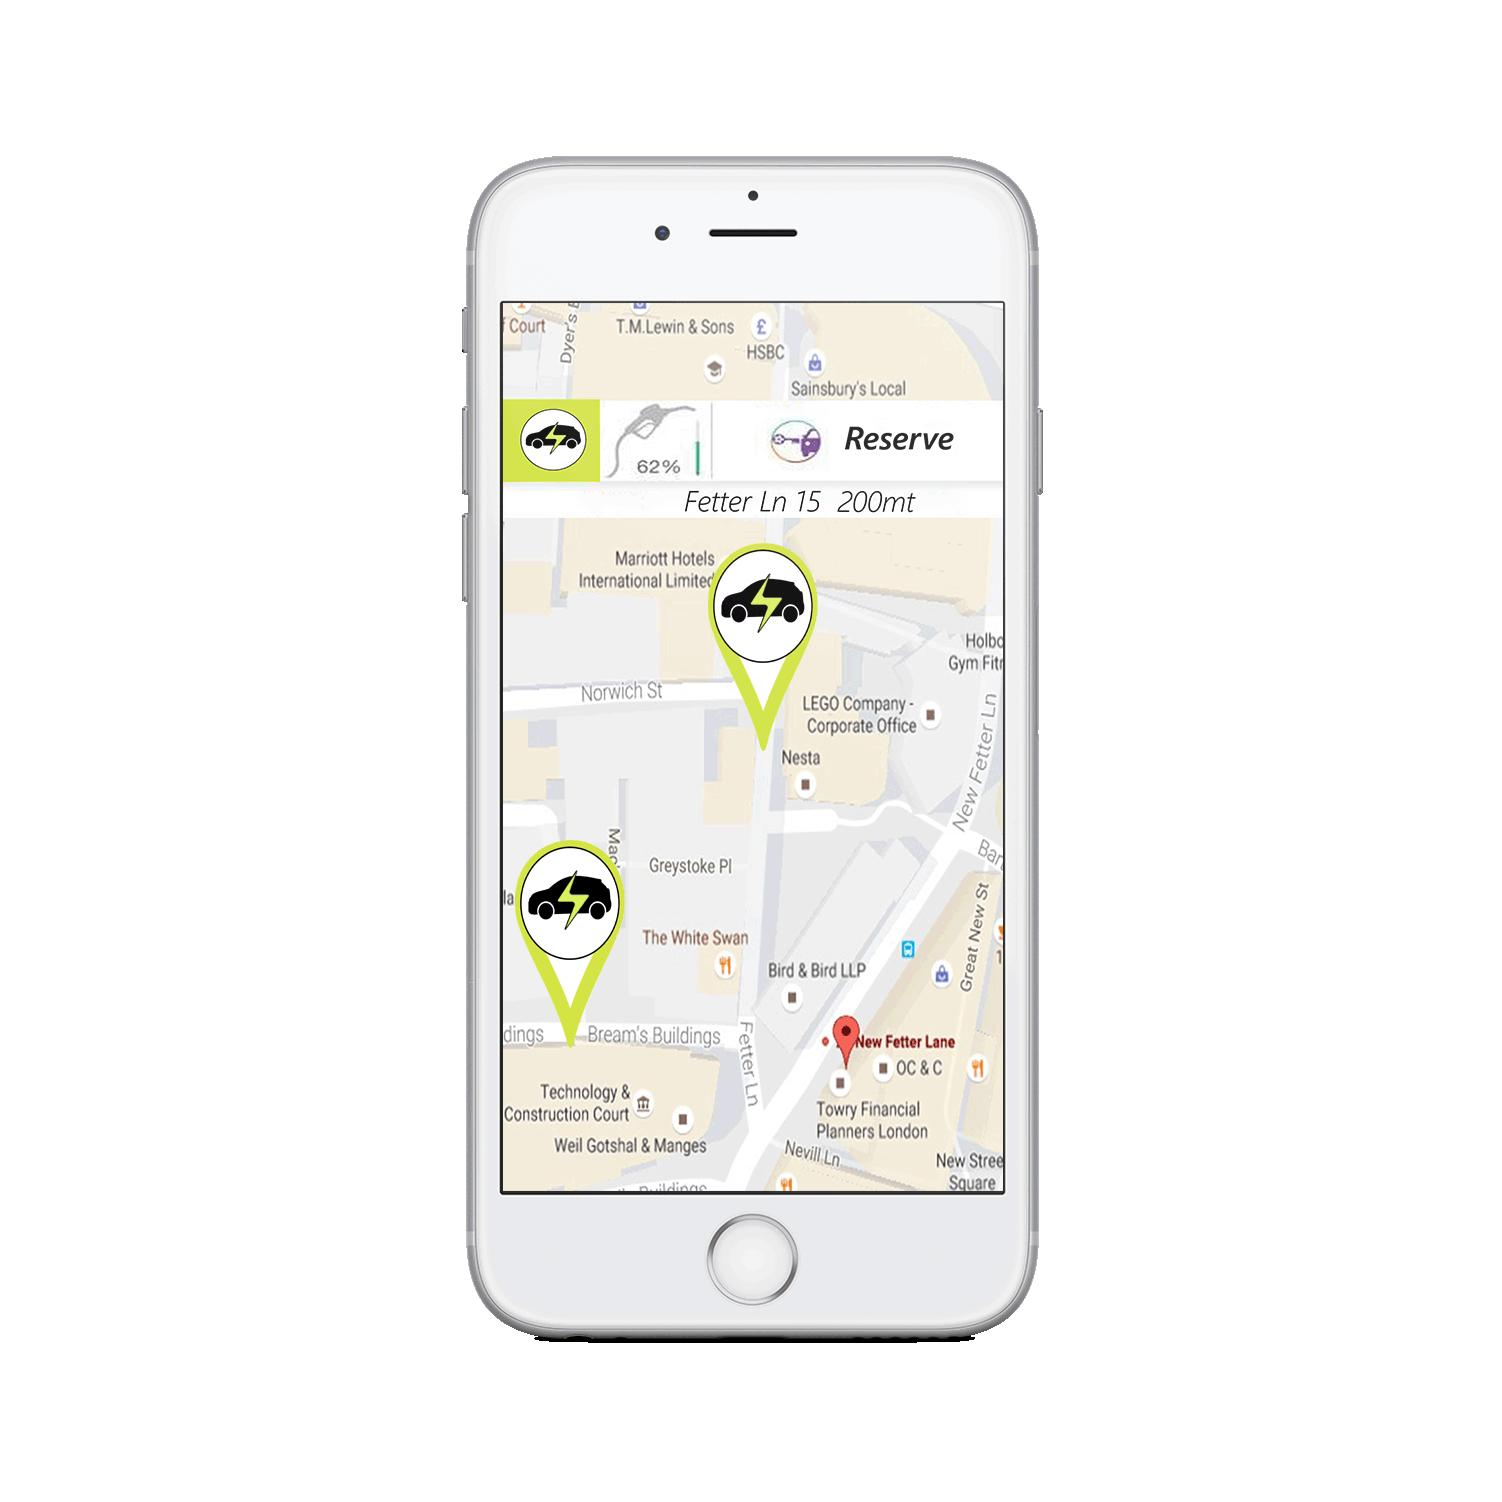
\includegraphics[width=400 pt]{resources/editato.jpg}
\caption{\label{fig:editato}View available car information in mobile application.}
\end{figure}

\subsubsection{View map on the website} This mockup shows the map that a generic user (guest or client) can see on the PowerEnJoy website.On the map are displayed the boundaries of the safe area in which a client can leave the car and the charging stations with the number of available charging spots.The user can insert an address in order to see the available cars within a certain distance.
\begin{figure}[h]
\centering
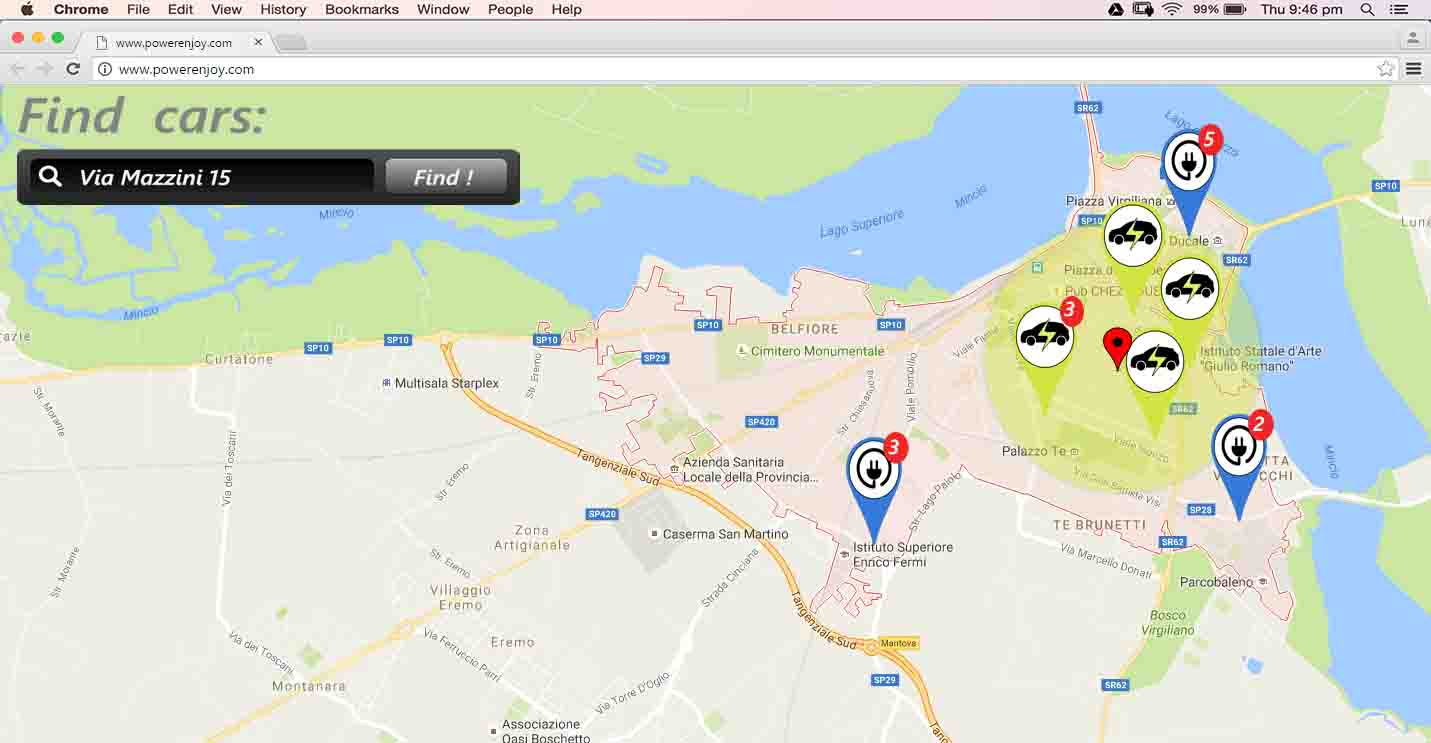
\includegraphics[width=450 pt]{resources/mappa.jpg}
\caption{\label{fig:mappa}View map on the website.}
\end{figure}

\subsubsection{Registration form} The mockup above shows the registration procedure that a guest has to complete in order to become a client and have access to the PowerEnJoy car sharing.

\begin{figure}[h]
\centering
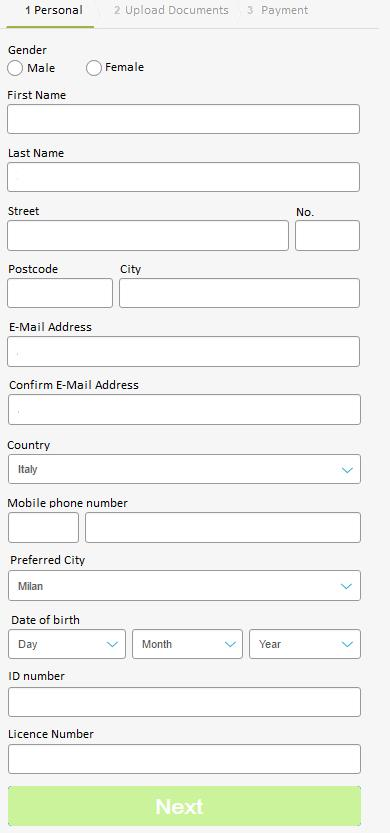
\includegraphics[height=200 pt]{resources/registrazione.jpg}
\caption{\label{fig:reg}Registration form.}
\end{figure}

\subsubsection{Insert pin on the car display} This mockup shows the form in which the client has to insert his pin. After inserting the correct pin the client can start the engine of the car.

\begin{figure}[ht]
\centering
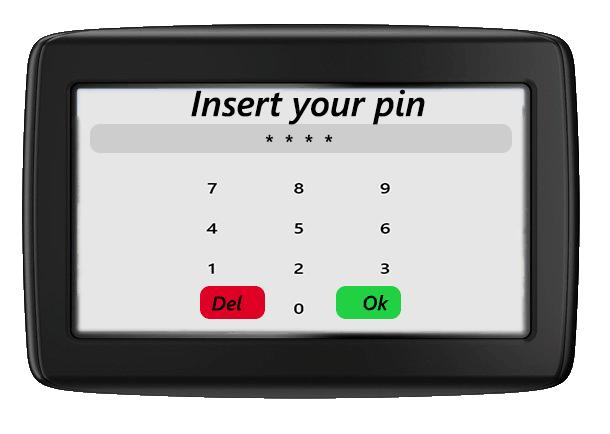
\includegraphics[width=400 pt]{resources/nav68.jpg}
\caption{\label{fig:pin}Insert pin on the car display.}
\end{figure}

\subsection{The world and the machine}

“The World and the Machine” model by M. Jackson and P. Zave is useful to identify the entities in the portion of system that has to be developed (\textbf{The Machine}) , the entities inside the portion of the real-world affected by the Machine (\textbf{The World}), and all  the \textbf{Shared Phenomena} that are controlled by the world and observed by the machine  or controlled by the machine and observed by the world.

\begin{figure}[ht]
\centering
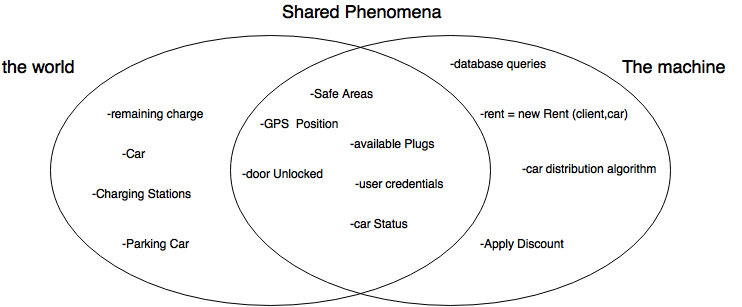
\includegraphics[width=400 pt]{resources/worldMachine.png}
\caption{\label{fig:WandM}The World and the Machine.}
\end{figure}
